\subsection{Unconstrained MPC - Closed Loop Simulation}
In this section the unconstrained MPC is simulated on both the linear and non-linear system. For this simulation, the tuning is set to $Q=100$ and $S=0.01$. It should be noticed that the values shown in the plot is absolute values.
\begin{figure}[H]
    \centering
    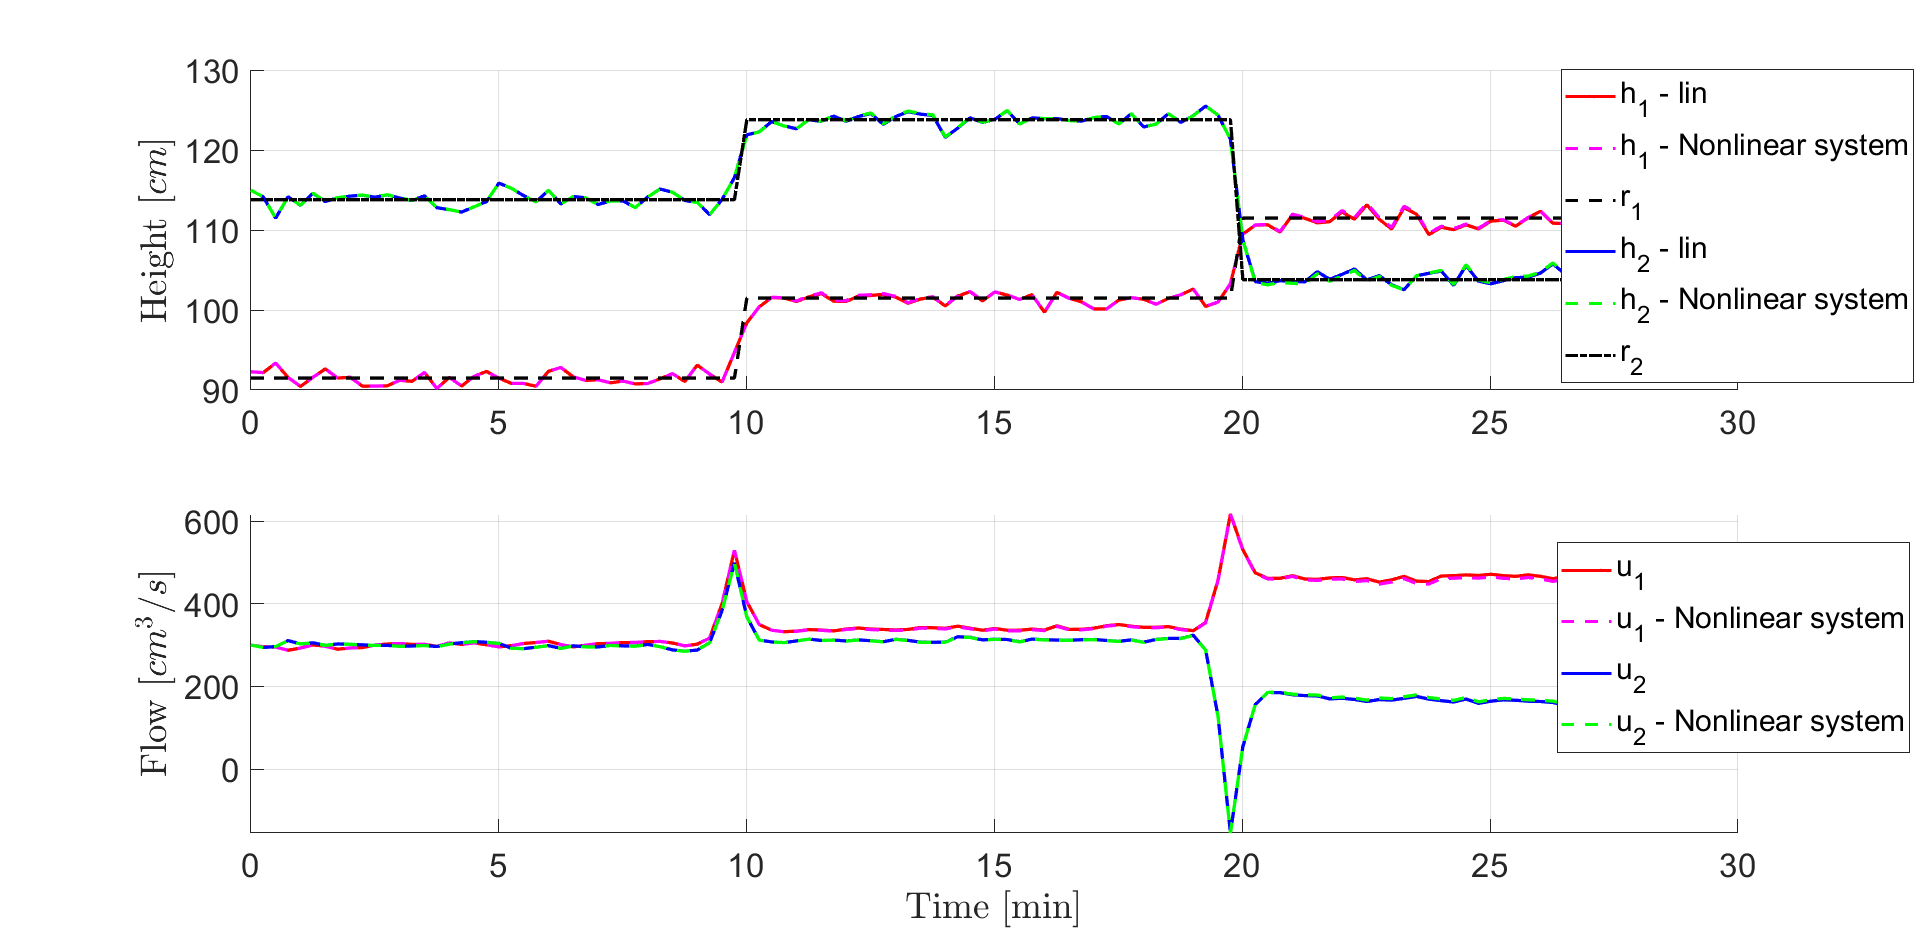
\includegraphics[width=1\textwidth]{Figures/Pr10.1_Uncon_MPC.png}
    \caption{Unconstrained MPC - Simulation on linear and non-linear model}
    %\label{fig:Kalman_stoc_state_step}
\end{figure}
It can be seen that the response of the linear and non-linear system with the linear unconstrained MPC is quite similar. However, if one zooms in minor deviations can be seen, specially close to the steps (I would have expected to have a larger deviation, but could not figure out why it didn't appear). The MPC is able to track the reference signal fast, however it is clear that the inputs are relatively high and fast changing. Wheen evaluating $u_2$ at $t=20\,[min]$ it is seen that the at negative flow is of course not realistic, but it is a consequence of the lack of constraints. 